\documentclass{standalone}
\usepackage{pgfplots}
\begin{document}
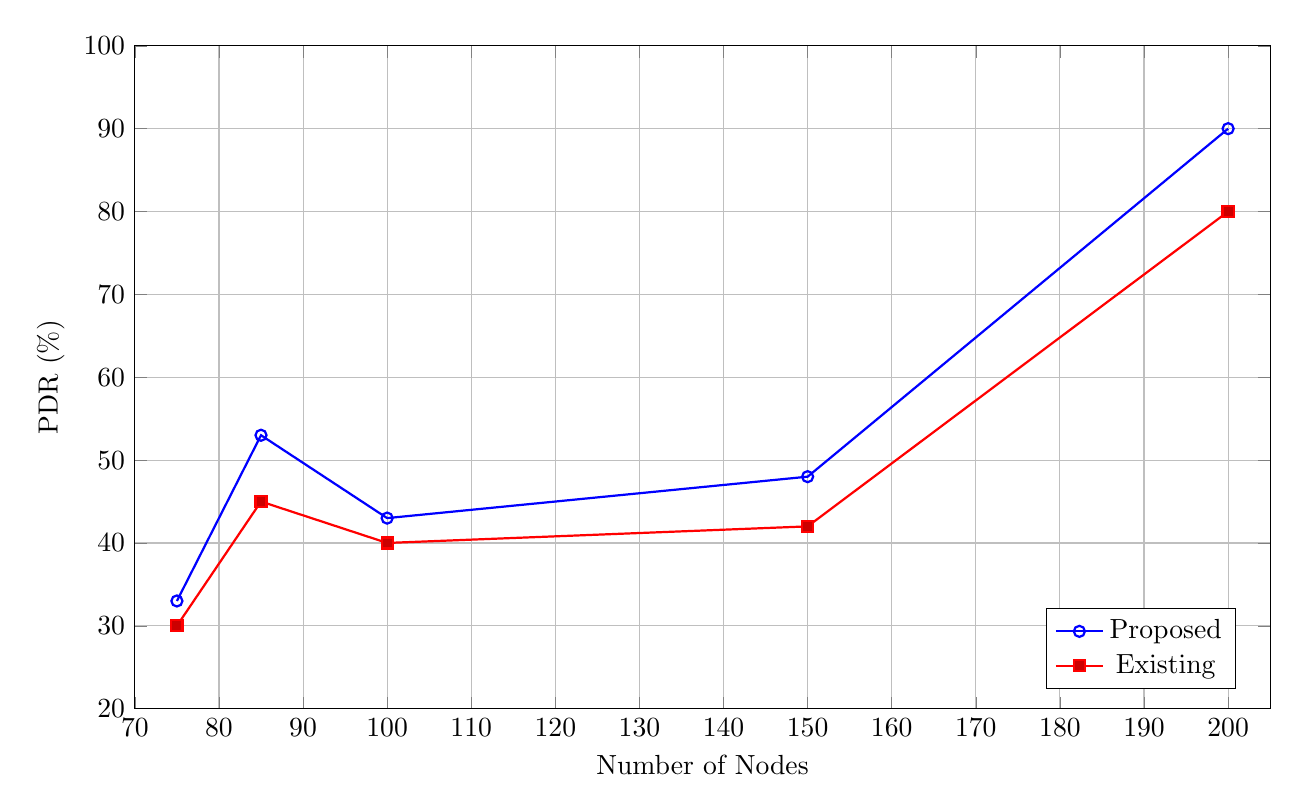
\begin{tikzpicture}
\begin{axis}[
width=16cm,height=10cm,
xlabel={Number of Nodes},
ylabel={PDR (\%)},
xmin=70,xmax=205,
ymin=20,ymax=100,
grid=major,
legend pos=south east
]
\addplot+[mark=o,thick] coordinates {
(75,33)(85,53)(100,43)(150,48)(200,90)
};
\addplot+[mark=square*,thick] coordinates {
(75,30)(85,45)(100,40)(150,42)(200,80)
};
\legend{Proposed,Existing}
\end{axis}
\end{tikzpicture}
\end{document}